%% LaTeX template for BSc Computing for Games final year project dissertations
%% by Edward Powley
%% Games Academy, Falmouth University, UK

%% Based on:
%% bare_jrnl.tex
%% V1.4b
%% 2015/08/26
%% by Michael Shell
%% see http://www.michaelshell.org/
%% for current contact information.
%%
%% This is a skeleton file demonstrating the use of IEEEtran.cls
%% (requires IEEEtran.cls version 1.8b or later) with an IEEE
%% journal paper.
%%
%% Support sites:
%% http://www.michaelshell.org/tex/ieeetran/
%% http://www.ctan.org/pkg/ieeetran
%% and
%% http://www.ieee.org/

%%*************************************************************************
%% Legal Notice:
%% This code is offered as-is without any warranty either expressed or
%% implied; without even the implied warranty of MERCHANTABILITY or
%% FITNESS FOR A PARTICULAR PURPOSE! 
%% User assumes all risk.
%% In no event shall the IEEE or any contributor to this code be liable for
%% any damages or losses, including, but not limited to, incidental,
%% consequential, or any other damages, resulting from the use or misuse
%% of any information contained here.
%%
%% All comments are the opinions of their respective authors and are not
%% necessarily endorsed by the IEEE.
%%
%% This work is distributed under the LaTeX Project Public License (LPPL)
%% ( http://www.latex-project.org/ ) version 1.3, and may be freely used,
%% distributed and modified. A copy of the LPPL, version 1.3, is included
%% in the base LaTeX documentation of all distributions of LaTeX released
%% 2003/12/01 or later.
%% Retain all contribution notices and credits.
%% ** Modified files should be clearly indicated as such, including  **
%% ** renaming them and changing author support contact information. **
%%*************************************************************************


\documentclass[journal]{IEEEtran}

\usepackage{graphicx}
% to embed the file `myreferences.bib` in your `.tex` file
% Insert additional usepackage commands here
\usepackage{color}
\usepackage{listings}
\usepackage[table]{xcolor}

\setlength{\arrayrulewidth}{0.5mm}
\setlength{\tabcolsep}{10pt}
%\usepackage{courier} %caused problems for me

\lstloadlanguages{% Check Dokumentation for further languages ...
	C,
	C++,
	csh,
	Java
}

\definecolor{red}{rgb}{0.6,0,0} % for strings
\definecolor{blue}{rgb}{0,0,0.6}
\definecolor{green}{rgb}{0,0.8,0}
\definecolor{cyan}{rgb}{0.0,0.6,0.6}

\lstset{
	language=csh,
	basicstyle=\footnotesize\ttfamily, 
	numbers=left, 
	numberstyle=\tiny, 
	numbersep=5pt, 
	tabsize=2, 
	extendedchars=true, 
	breaklines=true, 
	frame=b,
	stringstyle=\color{blue}\ttfamily, 
	showspaces=false, 
	showtabs=true, 
	xleftmargin=17pt,
	framexleftmargin=17pt,
	framexrightmargin=5pt,
	framexbottommargin=4pt,
	commentstyle=\color{green},
	morecomment=[l]{//}, %use comment-line-style!
	morecomment=[s]{/*}{*/}, %for multiline comments
	showstringspaces=false, 
	morekeywords={  abstract, event, new, struct,
		as, explicit, null, switch,
		base, extern, object, this,
		bool, false, operator, throw,
		break, finally, out, true,
		byte, fixed, override, try,
		case, float, params, typeof,
		catch, for, private, uint,
		char, foreach, protected, ulong,
		checked, goto, public, unchecked,
		class, if, readonly, unsafe,
		const, implicit, ref, ushort,
		continue, in, return, using,
		decimal, int, sbyte, virtual,
		default, interface, sealed, volatile,
		delegate, internal, short, void,
		do, is, sizeof, while,
		double, lock, stackalloc,
		else, long, static,
		enum, namespace, string},
	keywordstyle=\color{cyan},
	identifierstyle=\color{red},
}
\usepackage{caption}
\DeclareCaptionFont{black}{\color{black}}
\DeclareCaptionFormat{listing}

\begin{document}
%
% paper title
% Titles are generally capitalized except for words such as a, an, and, as,
% at, but, by, for, in, nor, of, on, or, the, to and up, which are usually
% not capitalized unless they are the first or last word of the title.
% Linebreaks \\ can be used within to get better formatting as desired.
% Do not put math or special symbols in the title.
\title{%
	To What Degree can an AI Built With Expert Strategies be Effective Against Competition AI?} %\\
	%\large A Planning Approach to StarCraft AI}

%
%
% author name
\author{\IEEEauthorblockN{James Hellman\\}
\IEEEauthorblockA{Falmouth Games Academy\\
UK, Falmouth\\
Email: jh182233@falmouth.ac.uk\\}
}

% The paper headers -- please do not change these, but uncomment one of them as appropriate
% Uncomment this one for COMP320
\markboth{COMP320: Research Review and Proposal}{COMP320: Research Review and Proposal}
% Uncomment this one for COMP360
% \markboth{COMP360: Dissertation}{COMP360: Dissertation}

% make the title area
\maketitle

% As a general rule, do not put math, special symbols or citations
% in the abstract or keywords.
\begin{abstract}
Effective macro-management (the ability to create armies and expand bases), is essential to obtaining victory in Real-Time Strategy (RTS), in the research community many Artificial Intelligence's (AI's) have been created to handle this. One method is to use a design approach to create what is known as a build order, many of these build orders take from expert strategies used by real people in high ranking tournaments. Build orders can be ridged during games leaving little room for adaptation to the opponent's strategy. In this work, a collection of build orders will be used to create an AI and investigates the impact of build orders that effectively counter-strategies used by other AI's. A hypothesis is made here that the AI will only be effective in the early stages of the game and will be outmanoeuvred in late-game stages. Therefore the effectiveness of this AI will be measured its average time survived, with a high average being effective and a low average being ineffective. Whether the AI wins the matches will also be taken into account, a higher average win rate will allow the AI to face a greater challenge. Upon successful completion of this work, the AI will be submitted to one of three competitions.
\end{abstract}

\section{Introduction}
\IEEEPARstart{I}{nvestigating} the effectiveness of an AI can be done in many ways, and the measurement of this is highl dependant on the method that is focused on when cre  Artificial Intelligence can be defined as anything that gives the illusion of intelligence to an appropriate level \cite{AIBook}. In games, AI has been used in both single and multi-player environments to help create a more immersive, challenging and fun experience. One such area which AI is prominent is in the Real-Time Strategy (RTS) genre and since the call for more research to be made for AI in RTS games by Michael Buro in 2004 \cite{CallFor}, research in this area has exploded \cite{Survey}. This has given rise to the creation of many AI's in RTS games, from AI's that are built with pre-defined build orders \cite{Swen} to deep Neural Networks \cite{Deep} that can learn from game-play replays, which will be covered in more detail later on in the paper.

RTS is a great test bed in AI research for its complex systems, involving many areas of interest in planning, dealing with uncertainty, domain knowledge exploitation, task decomposition, spatial reasoning, and machine learning \cite{StarCraftBot}. Unlike turn-based strategy, RTS requires real-time decision making with imperfect information, the information is limited through the use of partial visibility of the map. Unless the AI scouts the map (Sends a unit around the map) and sees what the opponent is doing, then the AI will have no access to any strategic knowledge. This along with the non-deterministic nature of RTS, meaning it may not exhibit the same behaviour on each run, makes RTS one of the most challenging environments in which to create an AI \cite{Current}.

Since the release of StarCraft Brood War API it has been easier for Academics to research AI in StarCraft, this has also given rise to an educational value as part of AI related subjects in several Universities around the world \cite{Current}. One example of this is the University Delft (NL), which for one of its modules the students are required to create a StarCraft Bot \cite{NL}. From this three yearly competitions have been created to compete students AI's, the first of which was hosted by the University of California, Santa Cruz in 2010 as part of the AAAI Artificial Intelligence and Interactive Digital Entertainment (AIIDE) conference program \cite{AIIDE}. Another hosted at the IEEE Computational Intelligence in Games (CIG) conference \cite{CIG}, and the last one which is an ongoing stand-alone event is the Student StarCraft AI Tournament (SSCAIT) \cite{StarCraftBot}. Upon successful completion of this work, the AI will be submitted to one of these three competitions.

This paper is organised as follows, first StarCraft and what it is will be presented, followed by a review of the current methods being utilized by the research community in the development of StarCraft AI's. With a description on the research that this work will be using, this is proceeded by the method and tools that will be used to create the AI as well the metrics used to measure its effectiveness finishing with the hypothesis.


\section{StarCraft}
StarCraft the most popular RTS game of all time \cite{Current} is an RTS game developed by Blizzard Entertainment \cite{Blizzard}\cite{Release}, released in 1998. Later that year StarCraft: Brood War was released and took hold in the e-sports community and is still popular today. StarCraft 2: Wings of Liberty was released much later in 2010, with a complete visual overhaul, most of the game mechanics remained the same other than balance changes. The premise of StarCraft is to gather resources, build a base, and build an army to then use to destroy an enemies base and army, during playtime, there are also many upgrades available for these units to give them the edge over an enemy who did not spend the time acquiring them. There are many ways of doing this each player with a different order of building their armies/bases commonly referred to as their "Build Order" \cite{BuildOrder}. Build orders refer to a players macro-management, whereas in StarCraft Micro-management is a huge part of the game, as those with greater control over individual units can better outmanoeuvre their opponent, and thus defeat them. There is a difference in the way units are controlled, in StarCraft:BW you can only select up to 12 units at a time and can not group them for easy selection, so when playing you have to utilise micromanagement skills more than in StarCraft 2 where you can select an unlimited number of units and can group them for easy selection.

\section{Related Work}
StarCraft is considered difficult due to its requirement of abstraction level thinking when planning. Strategy selection is perhaps the most important choice any player or AI can make in StarCraft and RTS as a whole, as this will dictate the actions and reactions which they take during playtime. Though a human player can be proficient at choosing their strategy by simply scouting the map, finding the enemy and seeing what they are building. The human player can then counter accordingly, and if they countered incorrectly the human player can simply change their strategy to accommodate. Creating an AI to do the same though can be a huge and complex task \cite{Fuzzy}\cite{OnlineEvo}\cite{GoalDriven}, one way to achieve this result without a large commitment of time is to create a library of expert strategies, and allow the AI to select the appropriate one throughout the game. This can be achieved using tools such as Advanced Behaviour Oriented Design Environment (ABODE) and Parallel-rooted Ordered Slip-stack Hierarchical (POSH) reactive plans \cite{POSH}, which will also be covered later in the paper. These tools allow for an iterative design approach for AI's in games and in this work will be focusing on the macro-management with a particular focus on build orders and the selection of strategies rather than micro-management. 

In the StarCraft research community, there are many different methods of AI creation. Some focus on micro-management like S. Liu et al \cite{EffectiveMicro} that uses a Genetic Algorithm (GA) and others that focus on macro-management looking at the build order like N. Justesen et al \cite{OnlineEvo}. Many of these research methods are cross depended and utilise more than one method, for example, D. Churchill et al \cite{Agents} created the UAlbertaBot, which was intended to automate both build order planning and unit control. There are also AI's that only use one strategy that has won several times in competitions like the ZZZKBot \cite{ZZZK}\cite{Results}, which only uses a 3pool build and built that uses a rush tactic. This rush tactic involves creating many weak inexpensive units and sending them to the enemy base within 5 minutes of starting the game. Many AI tend to struggle with countering this strategy, hence why this type of AI tends to win.

\subsection{Datasets}
A Dataset can be a collection of any data, for game AI a dataset can consist of thousands of replays with millions of game frames, and player actions\cite{Dataset}. This information can then put together to create a full game-state which allows for machine learning tasks \cite{Dataset17}. In AI research, datasets can be used in many approaches of development, one such use is to recreate game-states and evaluate them for prediction in realistic conditions \cite{SpecialTactics}.

\subsection{Micro-Management}
Micromanagement is a fundamental side of StarCraft game-play and many papers have their own approach to this aspect of RTS \cite{SOMA}\cite{EffectiveMicro}\cite{Swarm}\cite{MM}\cite{SpecialTactics}\cite{UnitsControl}. Micromanagement is the control of each unit individually, for example: if you have 12 units, each with their own ability, during battle you need to activate each ability at the correct time for each of the 12 units in order to utilise them to their full potential. This required you to select each unit during battle and activating the ability, while still maintaining control over the other 11 units. Though this is a slight exaggeration as in StarCraft some units have an auto use of their ability which allows the unit to decide when to use their ability, one such unit being the medic on the Terran faction which will heal any biological unit with less than full health. Also in StarCraft units can be selected by type i.e. you can double-click on a marine, and it will select all the marines on screen (Up to a maximum of 12). Players that perfect multitasking micromanagement skills are most likely to win the battles when playing, as they can outmanoeuvre their opponent much more easily and use abilities effectively to devastate their opponents armies. Many of these approaches tend to use either Genetic Algorithms (GA) or Evolutionary Algorithms (EA) \cite{SOMA}\cite{EffectiveMicro}\cite{Swarm}, while others observe replays and apply a Monte-Carlo method to create data for practice use \cite{MM}. But most of these methods have one thing in common, they all use a version of machine learning \cite{Survey}.

\subsection{Predictive Methods}
On a higher strategic level, the prediction of the opponent's strategy is a prominent approach used in research \cite{DataMine}\cite{Bayesian}\cite{Scouting}\cite{ReplayPred}. This type of research relies on the use of replays and machine learning to help the AI accurately predict a strategy, these do rely on the quantity and quality of replays used for the learning process\cite{DataMine}\cite{Bayesian}\cite{ReplayPred}. Another method for prediction is scouting alongside machine learning, this eliminates the need for replay observation and allows for a more real-time prediction \cite{Scouting}. Though this method does still require several games to be played before the AI can begin to have an accurate prediction.

Bayesian approaches are based on Bayes' Theorem which is another prediction method. Bayes' Theorem is a calculation of probability or also known as a probabilistic model \cite{BayesianAI}. In papers by G. Synnaeve et al \cite{UnitsControl}\cite{SpecialTactics} they create an AI that controls units individually, they do this by using uncertainty which instead of asking where a unit might be, it makes rough estimations and acts upon that. Another use for the Bayesian approach is to predict strategies, by creating a probabilistic model that after learning from replays can predict an opponent's strategy and adapt accordingly \cite{Bayesian}. A major downfall of Bayesian Approaches is that it can be computationally intense to calculate.

\subsection{Full Game Play}
Many papers try to create an AI capable of handling all aspects of an RTS \cite{Agents}\cite{Hierarchical}\cite{HumanLevel}\cite{SCAIL}. These AI's tend to take several methods that have been created in other research and combining them to form a new AI \cite{Agents}. Another use for the full gameplay AI is to try and create a "Human-Like" AI, which can mimic the play-style of an expert human player. Though the current AI's are limited in this as players reported that the AI's used unusual unit movements or building placement \cite{EvalHuman}.

\subsection{Neural Networks}
Neural Networking are computational models loosely based on the functioning of biological brains \cite{Deep}. Given an input it computes an output by using a large number of neural units, in StarCraft it can be used to predict strategies or in the case of StarCraft 2 with its new architecture it can be used for full game-play. Using a neural network would be impractical for the purpose of this work as it would take many months to train, and even then would not have a great chance of doing well against other AI's.

\subsection{Planning}
Planning in StarCraft usually deals with the build order that the AI will use usually only dealing with macro-management. There are several different ways to use a build order, some will use a static build order that will not change throughout the game \cite{Swen}, and the more popular route is to allow the AI to jump between build orders during play-time, another term is Reactive Planning \cite{Fuzzy}\cite{OnlineEvo}\cite{GoalDriven}. there has been some work on creating the build orders on the fly by finding out that most optimal method of gathering resource and building units \cite{BuildOrder}. Planning is perhaps the most optimal approach to creating an AI as there are little real-time calculations to make. Through the use of POSH tools \cite{POSH}, you can iteratively design AI prototypes and deploy quickly \cite{Swen}. 

From looking at the research in the field there are many methods that can be used to create an AI. The use of replays to train an AI to counter strategies can be effective \cite{Bayesian}, they lack the greater control of the game, the ability to macro-management as there are too many variables to consider. This lack of large-scale control is usually due to the heavy computational requirements of controlling each individual component of the game.  Due to this slow process, it is quite impractical to use when there is already a library of knowledge that can be to exploited \cite{Liquid}. Though there are AI's out there with planned strategies already programmed into them \cite{ZZZK}\cite{Fuzzy}, their limitation is that they only use a small number of strategies, though these work it can leave a lot of room for the opponent to manoeuvre. A logical step here is to program a larger pool of expert knowledge into the AI, it will then select one and follow it through, with the ability to jump between strategies at key points in-case a counter is detected. 

\subsection{StarCraft AI's}
In the StarCraft AI community there are many AI's that have been created to compete against each other, and in this work, a competition AI is defined as an AI that has been entered to the AI for Interactive Digital Entertainment conference (AAIDE) StarCraft AI Competition. A yearly competition hosted by David Churchill and sponsored by AIIDE. AI's in this grade include:
\begin{itemize}
\item ZZZKBot Winner of the 2017 AIIDE StarCraft AI Competition \cite{ZZZK}
\item Iron Winner of the 2016 AIIDE StarCraft AI Competition \cite{Iron}
\item UAlbertaBot Winner of the 2013/2011 AIIDE StarCraft AI Competition \cite{UAlberta}
\item Skynet Winner of the 2012 AIIDE StarCraft AI Competition \cite{Skynet}
\end{itemize}

These AI's use several strategies along with different factions and were chosen as they have all previously won the AIIDE StarCraft AI competition \cite{Results}.

\section{Method}
This work will be focusing on the implementation of an AI with pre-built build orders and their counters taken from Liquipedia \cite{Liquid}, a website dedicated to StarCraft, on the there they have a collection of strategies that are free to use in any capacity. Building upon these build orders the experiment will also include a method for swapping between the orders at any point, to know when to do this, the AI will scout the map in search of the opponent and compare their current building to its stored build orders and find an appropriate counter. The issue with this method is that in late game the AI will struggle to decide which build order to continue. 

\subsection{Tools}
There are several tools that will be using in this experiment, these include The Brood War Application Programming Interface (BWAPI), POSH tools, specifically POSH Sharp which is an interface that uses c\# instead of C++, and the ABODE editing software which uses POSH plans to create Behaviour Oriented Designs for AI's. 

\begin{figure}
\centering
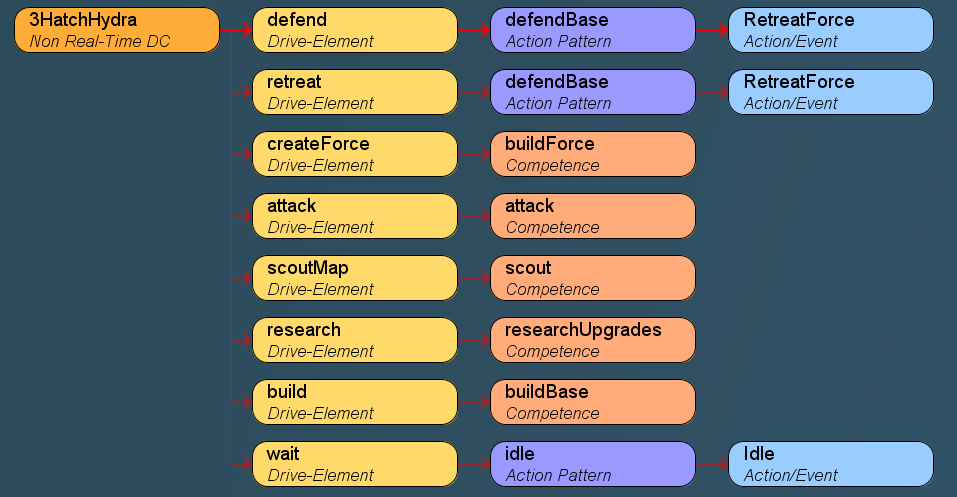
\includegraphics[width=0.5\textwidth]{POSH}
\caption{POSH plan for the Three Hatch Hydra build plan inside the ABODE editor.}
\label{Fig1}
\end{figure}
\begin{itemize}
\item \textbf{Brood War Application Programming Interface} \cite{BWAPI} is an open source software that creates an interface for a custom AI to use to communicate with the game. BWAPI deliberately does not give access to all the games information \cite{POSH}, limiting the AI to only be able to have information on the enemy if there is no Fog-of-War currently covering them, as well as the size of the map and base locations. This prevents custom AI's from cheating and ensures a fair game, though this could be considered a plus as it means that the developers of these AI's do not need to worry about using information that could cause their AI to cheat. Though this does mean that all the AI's must work in an imperfect environment which forces the AI to have to scout for information.
\item[]
\item \textbf{POSH} plans can be created in the ABODE Environment as seen in Figure 1, these are visual planning tools that allow for a hierarchy of actions with associated triggers. Each plan can be split into three parts, Drive-Collections, Competencies and Action patterns, these three determine when an action is to be triggered. POSH plans use a behaviour library created in the native language of the problem space, see Fig 2. 
\end{itemize}

\begin{figure}[h!]
\begin{lstlisting}
[ExecutableAction("SelectExtractorLocation")]
public bool SelectExtractorLocation()
{
    // enough resources available?
    if (!CanMorphUnit(bwapi.UnitTypes_Zerg_Extractor) || !Interface().baseLocations.ContainsKey((int)Interface().currentBuildSite))
    return false;
    
    TilePosition buildPosition = Interface().baseLocations[(int)Interface().currentBuildSite];
    // are there any geysers available/visible?
    IEnumerable<Unit> geysers = Interface()
        .GetGeysers().Where(geyser => geyser.getResources() > 0);
    if (geysers.Count() < 1)
        return false;

    // sort by closest path for ground units from selected build base
    TilePosition closest = geysers
        .OrderBy(geyser => geyser.getDistance(new Position(buildPosition)))
        .First().getTilePosition();

    // if there is a close geyers we are done
    if (closest is TilePosition)
    {
        this.buildLocation = closest;
        builder = Interface().GetBuilder(buildPosition);
        //move(new Position(closest), builder);
        // if (builder.getDistance(new Position(closest)) < DELTADISTANCE)
        //     return true;
        return true;
    }
    return false;
}	

\end{lstlisting}
\caption{c\# behaviour code snippet for selecting an extractor location for the Zerg, these behaviours are referred to by the POSH plan which determines when they are executed.}
\label{Fig2}
\end{figure}

\subsection{Process}
The first thing that will be chosen in the creation of this AI is to pick a faction, in StarCraft, there are three, Zerg, Protoss and Terran, each with their own unique play style. Zerg is a rushing faction, with their units being relatively weak and cheap usually focus on overwhelming their enemy with numbers. Protoss are strong but expensive, relying on smaller numbers and taking longer to produce anything means they can be weak at rushing and defending from a rush. Terran is a balance of the two, being able to produce strong and expensive units as well as cheap weak ones, they can effectively rush and defend from a rush.

In this work Protoss will be chosen, this choice was made as Zerg have been done many times and usually rely on rushes to win, whereas Terran are too complex for the planned AI. Protoss proved a happy middle ground to build upon where rushes are difficult to achieve but they are not too complex that it is too difficult to execute a sound strategy. So the second logical step is to implement an anti-rush strategy as an opening strategy. From there more aggressive strategies will be implemented and executed at the appropriate times. The challenge here is that it is difficult for Protoss to counter a Zerg rush but if successful it will leave the Zerg open for attack.

At each implementation, a test will be made on the AI to show its effectiveness and influence the next iteration of strategy implementation. These tests will consist of 10 games against the in-game AI until it has a relatively high win rate, at which point it will be tested against one of the competition AI's.


\subsection{Metrics}
In this work the StarCraft AI will be measured on its success using two factors:
\begin{itemize}
	\item Time Survived (Average of 13 minutes or above)
	\item End game Condition (Whether the AI wins the game or looses)
\end{itemize}

The average time of each game in the most recent StarCraft AI competition was 13 minutes, with the quickest average being 8 minutes and the longest being 19 minutes. The win ratio of the AI's vary substantially from 17.21\% to a high 83.11\% as can bee seen in Table 1 \cite{Results}. 

This AI will be considered effective if it can survive past the 13 minute mark, unless it wins the match at an earlier time.

Through these factors, the effectiveness of the AI will be determined, if the AI survives past the 13 minute average time or wins the game it will support a greater effectiveness. Though if the AI does not survive past the lower limit of 8 minutes or loses the Ai will need to be improved and tested again. 
To begin with, the AI will be pitted against the inbuilt AI as a test-bed, playing 10 matches against the three races. 10 being chosen as if the AI should win each game and or survive well into the upper range then there will be little reason to continue testing against the inbuilt AI as it will most likely continue this way. After the initial testing the AI will then be put against an open source competition grade AI, and 100 games for each AI will be simulated. This number has been chosen as it will give a total of 400 games and will proved strong evidence to support the hypothesis presented here.

\subsection{Hypothesis}

\begin{itemize}
	\item \textbf{Hypothesis 1} The AI will survive no less than 13 minutes in a match with the inbuilt AI.
	\item \textbf{Hypothesis 2} The AI will survive no less than 13 minutes in a match with the competition AI.
	\item \textbf{Hypothesis 3} The AI will defeat the inbuilt AI
	\item \textbf{Hypothesis 4} The AI will defeat the competition AI.
	\item \textbf{Hypothesis 5} The AI will counter the Rush tactic.
\end{itemize}


% references section

\bibliographystyle{IEEEtran}
\bibliography{references}

% Appendices
\appendix

\begin{table*}
	\centering
	{\rowcolors{3}{green!80!yellow!50}{green!70!yellow!40}
		\begin{tabular} { |p{3cm}||p{1.5cm}|p{1.5cm}|p{1.5cm}|p{1.5cm}|p{1.5cm}|  } 
			\hline
			\multicolumn{6}{|c|}{2017 AIIDE StarCraft AI Competition} \\
			\hline
			Bot & Games & Win & Loss & Win\% & AvgTime\\
			\hline
			ZZZKBot	&	2966	&	2465	&	501	&	83.11	&	8:00	\\
			PurpleWave	&	2963	&	2440	&	523	&	82.35	&	13:27	\\
			Iron	&	2965	&	2417	&	548	&	81.52	&	14:19	\\
			cpac	&	2963	&	2104	&	859	&	71.01	&	9:45	\\
			Microwave	&	2962	&	2099	&	863	&	70.86	&	11:34	\\
			CherryPi	&	2966	&	2049	&	917	&	69.08	&	9:50	\\
			McRave	&	2964	&	1988	&	976	&	67.07	&	14:35	\\
			Arrakhammer	&	2963	&	1954	&	1009	&	65.95	&	11:37	\\
			Tyr	&	2966	&	1955	&	1011	&	65.91	&	13:09	\\
			Steamhammer	&	2964	&	1901	&	1063	&	64.14	&	10:32	\\
			AILien	&	2966	&	1729	&	1237	&	58.29	&	13:04	\\
			LetaBot	&	2955	&	1682	&	1273	&	56.92	&	16:48	\\
			Ximp	&	2962	&	1605	&	1357	&	54.19	&	18:46	\\
			UAlbertaBot	&	2968	&	1585	&	1383	&	53.4	&	10:54	\\
			Aiur	&	2965	&	1496	&	1469	&	50.46	&	13:51	\\
			IceBot	&	2955	&	1348	&	1607	&	45.62	&	17:16	\\
			Skynet	&	2958	&	1295	&	1663	&	43.78	&	11:40	\\
			KillAll	&	2965	&	1276	&	1689	&	43.04	&	10:56	\\
			MegaBot	&	2802	&	1200	&	1602	&	42.83	&	12:21	\\
			Xelnaga	&	2962	&	1099	&	1863	&	37.1	&	15:19	\\
			Overkill	&	2958	&	967	&	1991	&	32.69	&	18:00	\\
			Juno	&	2962	&	876	&	2086	&	29.57	&	14:07	\\
			GarmBot	&	2961	&	802	&	2159	&	27.09	&	15:21	\\
			Myscbot	&	2964	&	769	&	2195	&	25.94	&	13:41	\\
			HannesBredberg	&	2964	&	630	&	2334	&	21.26	&	14:09	\\
			Sling	&	2963	&	625	&	2338	&	21.09	&	16:21	\\
			ForceBot	&	2960	&	532	&	2428	&	17.97	&	15:10	\\
			Ziabot	&	2964	&	510	&	2454	&	17.21	&	10:08	\\
			Total	&	41398	&	41398	&	41398	&	49.98	&	13:23	\\
			\hline
		\end{tabular}
		\caption{Results of the 2017 AIIDE StarCraft AI Competition Sourced from the official website \cite{Results}}
		\label{table:1}
\end{table*}

% that's all folks
\end{document}
